

\tikzset{every picture/.style={line width=0.75pt}} %set default line width to 0.75pt        

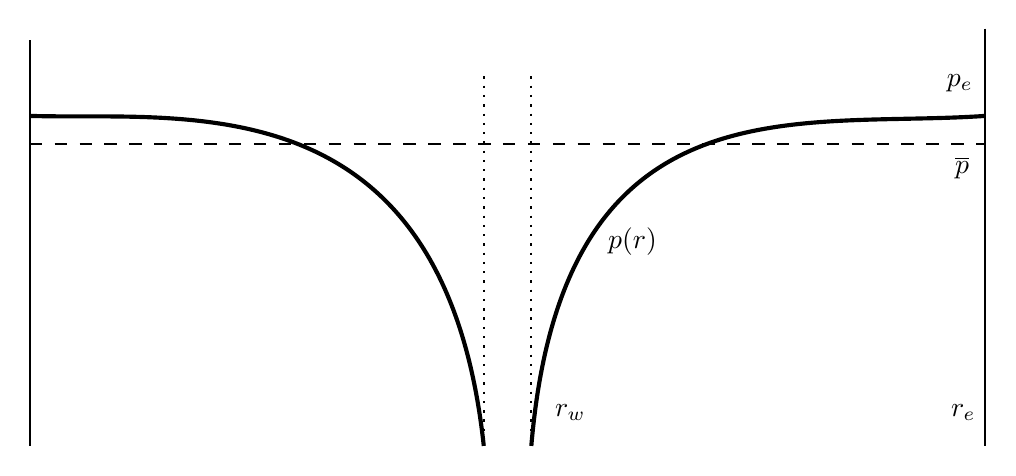
\begin{tikzpicture}[x=0.75pt,y=0.75pt,yscale=-1,xscale=1]
%uncomment if require: \path (0,300); %set diagram left start at 0, and has height of 300

%Curve Lines [id:da7511541250087521] 
\draw [line width=1.5]    (344.45,238) .. controls (359.67,59.33) and (472.6,85.33) .. (563.2,79) ;
%Curve Lines [id:da025905206061745956] 
\draw [line width=1.5]    (321.55,238) .. controls (302.33,60.67) and (177,81.33) .. (102.8,79) ;
%Straight Lines [id:da6790536850628852] 
\draw  [dash pattern={on 0.84pt off 2.51pt}]  (321.55,60) -- (321.55,238) ;
%Straight Lines [id:da4154351528354687] 
\draw  [dash pattern={on 0.84pt off 2.51pt}]  (344.45,60) -- (344.45,238) ;
%Straight Lines [id:da012417840094577581] 
\draw  [dash pattern={on 4.5pt off 4.5pt}]  (102.8,92.67) -- (563.2,92.67) ;
%Straight Lines [id:da923812897272561] 
\draw    (102.8,42.67) -- (102.8,238) ;
%Straight Lines [id:da9720690336089455] 
\draw    (563.2,37) -- (563.2,238) ;

% Text Node
\draw (354.45,216.4) node [anchor=north west][inner sep=0.75pt]    {$r_{w}$};
% Text Node
\draw (545.2,216.4) node [anchor=north west][inner sep=0.75pt]    {$r_{e}$};
% Text Node
\draw (543.2,57.4) node [anchor=north west][inner sep=0.75pt]    {$p_{e}$};
% Text Node
\draw (547.2,97.07) node [anchor=north west][inner sep=0.75pt]    {$\overline{p}$};
% Text Node
\draw (380,131.4) node [anchor=north west][inner sep=0.75pt]    {$p( r)$};


\end{tikzpicture}